\section{Substitution}
Recall that the chain rule for differentiation is given by
\begin{displaymath}
  \od{}{x} f(g(x)) = f'(g(x)) g'(x).
\end{displaymath}

In other words, $ f(g(x)) $ is an anti-derivative of $ f'(g(x)) g'(x) $ and so we can write
\begin{displaymath}
  \rint f'(g(x)) g'(x) \dif{x} = f(g(x)) + C.
\end{displaymath}

To make this rule easier to apply in practice, we often perform what is known as a change of variables. We
let $ u = g(x) $, and then $ \od{u}{x} = g'(x) $. Substituting this in, we obtain
\begin{displaymath}
  \rint f'(g(x)) g'(x) \dif{x} = \rint f'(u) \od{u}{x} \dif{x}
\end{displaymath}
and then the rule is just the statement that we can `cancel' the $ \dif{x} $'s, producing
\begin{displaymath}
  \rint f'(g(x)) g'(x) \dif{x} = \rint f'(u) \frac{\dif{u}}{\cancel{\dif{x}}} \cancel{\dif{x}} = \rint f'(u) \dif{u} = f(u) + C = f(g(x)) + C.
\end{displaymath}

This rule, which gives us a kind of chain rule for integration, is called \emph{substitution}, or the \emph{inverse chain rule}. It
can be thought of as a change in coordinate system from an $ x$-based system to one based on $ u $, and we have to `resize' our curve based
on how much $ u $ stretches the coordinate system compared to $ x $ --- and this `stretch factor' is simply $ \od{u}{x} $.

\begin{exs}\leavevmode
  \begin{enumerate}
    \item Suppose we wish to find $ \rint \sin x \cos x \dif{x} $. Then let $ u = \sin x $, so $ \dif{u} = \cos x \dif{x} $
          and
          \begin{displaymath}
            \rint \sin x \cos x \dif{x} = \rint u \dif{u} = \frac{1}{2} u^2 + C = \frac{1}{2} \sin^2 x + C.
          \end{displaymath}
          In this case, we also could have used a trigonometric identity.
    \item Suppose we wish to find $ \rint xe^{x^2} \dif{x} $. We can let $ u = x^2 $, and then $ du = 2x \dif{x} \Rightarrow \dif{x} = \frac{du}{2x} $.
          Hence:
          \begin{displaymath}
            \rint xe^{x^2} \dif{x} = \rint \frac{1}{2} e^u \dif{u} = \frac{1}{2} e^u + C = \frac{1}{2}e^{x^2} + C.
          \end{displaymath}
    \item Suppose we wish to find $ \rint \frac{4}{x} (\ln x)^3 \dif{x} $. We let $ u = \ln x $, and then $ \dif{u} = \frac{\dif{x}}{x} $.
          Hence:
          \begin{displaymath}
            \rint \frac{4}{x} (\ln x)^3 \dif{x} = 4\rint u^3 \dif{u} = u^4 + C = (\ln u)^4 + C.
          \end{displaymath}
  \end{enumerate}
\end{exs}

\subsection{Exercises and Problems}
\begin{enumerate}
  \item Find the following indefinite integrals. (Remember, the indefinite integral of $ f $, $ \rint f(x) \dif{x} $, is
        the family of anti-derivatives of $ f $.)
    \begin{multicols}{2}
    \begin{enumerate}
      \item $\displaystyle \rint \sin 2x \dif{x} $
      \item $\displaystyle \rint \tan x \dif{x} $
      \item $\displaystyle \rint 3x\cos x \dif{x} $
      \item $\displaystyle \rint \frac{\cos x}{\sin x + 1} \dif{x} $
      \item $\displaystyle \rint (4x - 44)^{2019} \dif{x} $
      \item $\displaystyle \rint 4x \sqrt{x^2 + 3} \dif{x} $
      \item $\displaystyle \rint (3x - 4)^2 \dif{x} $
      \item $\displaystyle \rint \frac{x}{x^2 + 1} \dif{x} $
      \item $\displaystyle \rint \frac{2}{4x + 3} \dif{x} $
      \item $\displaystyle \rint e^{2x + 1} \dif{x} $
      \item $\displaystyle \rint \sec 4x \tan 4x \dif{x} $
      \item $\displaystyle \rint 2\cos x + \sin 2x \dif{x} $
      \item $\displaystyle \rint -2x\csc^2 (3x^2) \dif{x} $
      \item $\displaystyle \rint \frac{3}{x^3} - \frac{4}{x + 1} \dif{x} $
      \item $\displaystyle \rint e^{x/2} + \frac{2}{x} \dif{x} $
      \item $\displaystyle \rint x^2 \sec^2 x^3 + 9 \dif{x} $
      \item $\displaystyle \rint -\csc (\tan x) \cot (\tan x) \sec^2 x \dif{x} $
      \item $\displaystyle \rint \frac{\cos x - \sin x}{\cos x + \sin x} \dif{x} $
      \item $\displaystyle \rint \frac{2017}{x\ln x} \dif{x} $
      \item $\displaystyle \rint \tan x + \frac{1}{\tan x} \dif{x} $
      \item $\displaystyle \rint (\cos x) (\sin \sin x) (\cos \cos \sin x) \dif{x} $
    \end{enumerate}
    \end{multicols}
  \item By using the substitution $ x = \sin \theta $, find
        \begin{displaymath}
          \rint \frac{1}{\sqrt{1 - x^2}} \dif{x}.
        \end{displaymath}
  \item Evaluate $ \rint \cos^5 x \dif{x} $ using the substitution $ t = \sin x $.
  \item Find $ \rint \tan \theta \dif{\theta} $ and $ \rint \cot \theta \dif{\theta} $.
  \item Complete the following working:
        \begin{align*}
          \rint \sec x \dif{x} &= \rint \sec x \frac{\sec x + \tan x}{\sec x + \tan x} \dif{x}\\
                              &= \rint \frac{\dots}{\sec x + \tan x} \dif{x}\\
                              \text{Let $ u = \dots $}\\
                              &= \rint \frac{1}{\dots} \dif{u}\\
                              &= \dots
        \end{align*}
  \item Find an anti-derivative of $ \csc x $. (Hint: consider the previous problem.)
  \item The velocity of a particle at time $ t $ is given by $ v = \dfrac{\cos(\sqrt{2t + 1})}{\sqrt{2t + 1}} $.
        What is the position of the particle at time $ t = 5 $, given that $ x(0.5) = 0 $? (Recall that $ v = \od{x}{t} $.)
  \item Consider the following indefinite integral:
        \begin{displaymath}
          \rint \frac{1}{\sqrt{1 - x^2}} \dif{x}.
        \end{displaymath}
    \begin{enumerate}
      \item Show, using the inverse function rule for differentiation, that the anti-derivatives
            of $ \frac{1}{\sqrt{1 - x^2}} $ are $ \sin^{-1} x + C $.
      \item Compute the indefinite integral a different way, using the substitution $ x = \sin \theta $.
      \item Find the anti-derivatives of
            \begin{displaymath}
              f(x) = \frac{-1}{2\sqrt{x - x^2}}.
            \end{displaymath}
            (Hint: try to substitute $ u = \sqrt{1 - x} $.)
    \end{enumerate}
  \item Compute the following:
    \begin{enumerate}
      \item $ \displaystyle\rint \dfrac{x^2(5x^2 + 4x - 3)}{x^5 + x^4 - x^3 + 1} \dif{x} $`
       \item $ \displaystyle\rint \dfrac{x^2 + 1}{x(x^2 + 3)} \dif{x} $
    \end{enumerate}
\end{enumerate}
The previous problem involved finding anti-derivatives of \emph{rational functions}: those of the form $ \frac{P(x)}{Q(x)} $
for polynomials $ P $ and $ Q $. In general, it is possible to find anti-derivatives of all such functions by writing them
as sums of fractions with linear or quadratic denominators; this is known as \emph{expansion via partial fractions}.
\begin{enumerate}[resume]
  \item Some more interesting problems:
    \begin{enumerate}
      \item Rewrite in the form $ \dfrac{A}{x-1} + \dfrac{B}{(x-1)^2} + \dfrac{C}{x + 1} $ and integrate:
        \begin{displaymath}
          \rint \dfrac{4x}{x^3 - x^2 - x + 1} \dif{x}.
        \end{displaymath}
      \item Use the obvious substitution and divide through:
        \begin{displaymath}
          \rint \dfrac{\sqrt{x+1}}{x} \dif{x}.
        \end{displaymath}
    \end{enumerate}
  \item Recall that $ \od{}{x} \tan^{-1} x = \frac{1}{x^2 + 1} $.
    \begin{enumerate}
      \item Rewrite the given rational function as follows:
            \begin{displaymath}
              \frac{x^2 + x - 2}{3x^3 - x^2 + 3x - 1} = \frac{A}{3x - 1} + \frac{Bx + C}{x^2 + 1}
            \end{displaymath}
      \item Hence (or otherwise) compute:
            \begin{displaymath}
              \rint \frac{x^2 + x - 2}{3x^3 - x^2 + 3x - 1} \dif{x}.
            \end{displaymath}
    \end{enumerate}
  \item Use appropriate substitutions to evaluate:
    \begin{enumerate}
      \item $ \displaystyle\rint \dfrac{\cos \theta}{\sin^2 \theta + 4 \sin \theta - 5} \dif{\theta} $
      \item $ \displaystyle\rint \dfrac{e^{3x}}{e^{2x} + 4} \dif{t} $
      \item $ \displaystyle\rint \dfrac{5 + 2\ln x}{x(1 + \ln x)^2} $
    \end{enumerate}
  \item In the following, let $ t = \tan \frac{x}{2} $ (where $ \abs{x} < \pi $). We will apply the techniques
        from the last few problems in the notes, calculating some anti-derivatives of rational functions by
        expanding them as sums of fractions.
    \begin{enumerate}
      \item Show that:
            \begin{displaymath}
              \cos\left( \frac{x}{2} \right) = \frac{1}{\sqrt{1 + t^2}} \quad\text{and}\quad \sin\left(\frac{x}{2}\right) = \frac{t}{\sqrt{1 + t^2}}
            \end{displaymath}
      \item Show that:
            \begin{displaymath}
              \cos x = \frac{1 - t^2}{1 + t^2} \quad\text{and}\quad \sin x = \frac{2t}{1 + t^2}
            \end{displaymath}
      \item Show that:
            \begin{displaymath}
              \od{x}{t} = \frac{2}{1 + t^2}
            \end{displaymath}
      \item Use the substitution $ t $ to evaluate:
        \begin{enumerate}
          \item $ \rint (1 - \cos x)^{-1} \dif{x} $
          \item $ \rint (3\sin x - 4\cos x)^{-1} \dif{x} $
        \end{enumerate}
    \end{enumerate}
\end{enumerate}

\subsection{References}
For exercises and notes on substitution, see Thompson chapter XX (the section on substitution
is two or three pages in). For partial fractions, see chapter XIII.

For the interested, a proof that one can always expand a rational function into partial fractions
is outlined as exercise 11.1.13 in Artin (p. 441).

\subsection{Homework}
\paragraph{Reading}
\begin{figure}
  \centering
  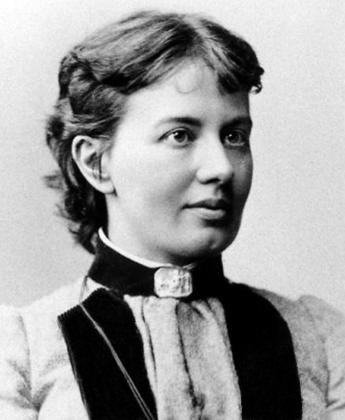
\includegraphics[width=0.2\textwidth]{kovalevskaya}
  \caption{Sofia Kovalevskaya (public domain)}
\end{figure}
Sofia Kovalevskaya (1850--1891) was the daughter of an artillery general and a member of the Russian
nobility. It so happened that her nursery walls had been papered with pages from lecture
notes on analysis. At the age of 11 she took a close look at her wallpaper and taught herself
calculus. She became attracted to mathematics, preferring it to all other areas of study.
Her father tried to stop her, but she carried on regardless, reading an algebra book
when her parents were sleeping.

In order to travel and obtain an education, she was obliged to marry, but the marriage was
never a success. In 1869 she studied mathematics in Heidelberg, but because female students
were not permitted, she had to pursuade the university to let her attend lectures on an
unofficial basis. She showed impressive mathematical talent, and in 1871 she went to Berlin,
where she studied under the great analyst Karl Weierstrass. Again, she was not permitted
to be an official student, but Weierstrass gave her private lessons.

She carried out original research, and by 1874 Weierstrass said that her work was suitable
for a doctorate. She had written three papers, on differential equations, elliptic functions,
and the rings of Saturn. In the same year G\"ottingen University awarded her a doctoral
degree. The differential equations paper was published in 1875.

In 1878 she had a daughter, but returned to mathematics in 1880, working on the refraction
of light. In 1883 her husband, from whom she had separated, committed suicide and she spend
more and more time working on her mathematics to assuage her feelings of guilt. She obtained
a university position in Stockholm, giving lectures in 1884. In 1889 she became the third
female professor ever at a European university, after Maria Agnesi (who never took up her
post) and the physicist Laura Bassi. Here she did research on the motion of a rigid body,
entered it for a prize offered by the Academy of Sciences in 1886, and won. The jury found
the work so brilliant that they increased the prize money. Subsequent work on the same topic
was awarded a prize by the Swedish Academy of Sciences, and led to her being elected to the
Imperial Academy of Sciences.

\begin{flushright}
  From \textit{Taming the Infinite}, by Ian Stewart (Quercus, 2008).
\end{flushright}


\paragraph{Problems}
\begin{enumerate}
  \item Calculate the following indefinite integrals:
    \begin{enumerate}
      \item $ \rint -\csc 3x \cot 3x \dif{x} $
      \item $ \rint -x\sec^2 3x^2 \dif{x} $
      \item $ \rint \frac{\sqrt{x} + 3x - 2}{x} \dif{x} $
      \item $ \rint \sin^3 x \cos^2 x \dif{x} $ (Hint: use $ \sin^2 x = 1 - \cos^2 x $ to rewrite the integrand.)
    \end{enumerate}
  \item Recall that $ \od{}{x} \tan^{-1} x = \frac{1}{1 + x^2} $. Find $ \rint \frac{x}{1 + x^4} \dif{x} $.
  \item Let $ y $ be a function of $ x $, and let $ x $ in turn be a function of $ t $. If $ \od{y}{x} = 3 $ when $ x = 0 $,
        and if $ x(t) = 7t + e^t $, find an explicit expression for $ y(t) $.
\end{enumerate}
